
\documentclass[journal,UTF8]{IEEEtran}
%\usepackage{ctex}
\usepackage{color}

%
\usepackage{cite}

\ifCLASSINFOpdf
 \usepackage[pdftex]{graphicx}
  % declare the path(s) where your graphic files are
 \graphicspath{{../pdf/}{../jpeg/}}
  % and their extensions so you won't have to specify these with
  % every instance of \includegraphics
\DeclareGraphicsExtensions{.pdf,.jpeg,.png}
\else
  % or other class option (dvipsone, dvipdf, if not using dvips). graphicx
  % will default to the driver specified in the system graphics.cfg if no
  % driver is specified.
\usepackage[dvips]{graphicx}
  % declare the path(s) where your graphic files are
\graphicspath{{../eps/}}
  % and their extensions so you won't have to specify these with
  % every instance of \includegraphics
\DeclareGraphicsExtensions{.eps}
\fi

\usepackage[cmex10]{amsmath}

%\usepackage{algorithmic}
\usepackage[ruled]{algorithm2e}
\usepackage{array}

\ifCLASSOPTIONcompsoc
  \usepackage[caption=false,font=normalsize,labelfont=sf,textfont=sf]{subfig}
\else
  \usepackage[caption=false,font=footnotesize]{subfig}
\fi

\hyphenation{op-tical net-works semi-conduc-tor}



\begin{document}
%
% paper title
% can use linebreaks \\ within to get better formatting as desired
% Do not put math or special symbols in the title.
\title{A VCA Protocol Based Multi-level Flexible Architecture on Embedded PLCs for Visual Servo Control }

\maketitle

\begin{abstract}
The visual system, motion control system and programmable logic controller (PLC) system are becoming increasingly inseparable, however there are few papers discussing the integration of these three systems. Most of papers are focusing on their applications individually. We propose a flexible multi-level architecture which is based on a $VCA$ protocol to address the integration problem. The multi-level includes flexible layer, control layer and algorithm layer. The flexible layer is adopted to seamlessly integrate visual system and embedded PLC ($ePLC$) system. The $VCA$ protocol is designed to data interaction between the layers. Correspondingly, a customized hardware, memory allocation, multithreading structure are described to support the proposed flexible software architecture. At last, we implement two cases using the proposed $VCA$ protocol based flexible architecture in which the generality of the proposed flexible architecture is verified. In first case, the winding machine with visual system implements regular winding effect by the correction of $\theta$. In second case, the binocular catching robot uses the camera to track the trajectory and send to $ePLC$. By adjusting the speed and position, the robot can catch the ball finally.
\end{abstract}

% Note that keywords are not normally used for peerreview papers.
\begin{IEEEkeywords}
motion control, visual servo control, embedded PLC, multi-level architecture
\end{IEEEkeywords}

% For peer review papers, you can put extra information on the cover
% page as needed:
% \ifCLASSOPTIONpeerreview
% \begin{center} \bfseries EDICS Category: 3-BBND \end{center}
% \fi
%
% For peerreview papers, this IEEEtran command inserts a page break and
% creates the second title. It will be ignored for other modes.
\IEEEpeerreviewmaketitle



\section{Introduction}
Integration technologies are driving the industrial automation \cite{Kazmierkowski2007Integration}. The continuously integrations of sensors, controllers, robots, tools, etc. bring the concepts of self-aware equipment, intelligent factory and CPS, etc. \cite{Wan2018An,Chekired2018Industrial}. Recent researches \cite{Colombo2006An,Vaccaro2010An,Dean2017Integration} introduce the development of integration technologies. In industrial automation, PLC system,  motion control system and visual system become more and more important and inseparable \cite{Feng2002Integrating,Chang2006Motion,Feng2005Practical}. On the other hand, the advances of edge computing, fog computing and edge artificial intelligence \cite{Hu2017Fog,Hou2018Green,PaceAn} put forward new challenges on edge equipment of these systems.

\subsection{Motivations}
Recent advances in image processing and pattern recognition contribute to the thriving of visual system which has been applied in various fields. By extracting features from the image, the visual system could obtain parameters to replace human visual system to address lots of tasks, specially, the ever-growing requirements in industrial scenarios, e.g. works should be finished in dangerous environment, human vision is difficult to satisfy or numerous visual systems are needed in some large scale industrial production. 

After the visual processing, in most cases, the motion control system as the power of automation is constantly needed to drive some actuators to finished some severe tasks which remarkably benefit of the replacement of large labor force. 

On the other hand, PLCs have become a base of automation owning to its high reliability and easy programming\cite{Hossain2014Advanced}. Furthermore, Lots of researches are focusing on it to extremely extend its applied field. For instance, \cite{Jiang2013System,Jiang2013Bayesian} guarantee the reliability by verifying the program of PLCs, \cite{Gerk2006Advanced,Dominic2016PLC} improve the performance of PLCs using advanced algorithms, \cite{wu2018customized} alleviates the development complexity of PLCs with a special software structure, \cite{Sch2013Development} pose methods to update PLC programs dynamically.


In addition, the visual system, motion control system and PLC system are becoming increasingly inseparable. \cite{Chen2014A} is a typical case that describes how the three parts collaborate. The visual system analyzes the context and get error put into the motion control system. Simultaneously the PLC is judging the information, such as the position limitation of the every axis, to make some logical judgments accordingly. 

Hence, how to pose a flexible structure to the integration of visual system, motion control system and  PLC system attracts us.

\subsection{Related Works}

Visual control system is combined of special motion control system and visual system which is applied in various field, such as transport \cite{Xing2014Intersection}, circuit detection\cite{Nian2005An}, sorting system, welding\cite{Chen2014A}, assembling\cite{Wang2008Visual,Xiao2014Visual}, robot\cite{Wu2013Cloud,Tsai2017A}, unmanned aerial vehicles\cite{Guenard2010A,Serra2016Landing} and sorting\cite{Sun2013Automatic}. These works address their problems in relevant fields. However, all these solutions are based on special motion control system and visual system.

On the other hand. The integration of logic control and motion control has variously deep researches \cite{Ioannides2004Design,Shi2016The,Fang2017Design, syaichu2011model}. \cite{Ioannides2004Design,syaichu2011model} realize the motion control directly in PLC. \cite{Peng2011Linear, Qian2014A, OMRON2006CS1W} use motion control module collaborated with PLC to implement their applications. However, the development method in these papers is disordered. Therefore, in 2005, PLCopen organization has released a related standard \cite{PLCopen2005Function} which standardizes the motion control in PLC. Based on this standardization, \cite{S2006Advanced} provides an advanced implementation in distributed automation system and companies, such as 3S \cite{3S2017Logic}, provide some tools. \cite{wu2018customized} poses a customized real-time compilation method to reduce the development complexity.

Above works provide impressive integrations on visual servo control system and PLC with motion control functions, however there are few papers discussing the integration of visual system, motion control and PLC. Most of applications are focusing on their applications with three individual systems, such as \cite{Chen2014A}. Hence, an integration structure of PLC system, motion control system and visual system should be provided to reduce the complexity and expand the application fields.

\subsection{Our Contributions}
We propose a flexible multi-level architecture which is based on a $VCA$ protocol to address the problem of integration of PLC system, motion control system and visual system in ePLCs. The multi-level includes flexible layer, control layer and algorithm layer. The $VCA$ protocol is designed to data interaction between the layers. Correspondingly, a customized hardware, memory allocation, multithreading structure are described to support the proposed flexible software architecture.
In the remaining paper, in Section \ref{SystemStructure}, the hardware ans software structure, memory allocation and thread structure are introduced. In Section \ref{Integration}, the mechanism of $VCA$ protocol is addressed in detail. In Section \ref{Execution}, we illustrate the execution process of the proposed system. Then, we implement two cases which are binocular catching robot and winding machine with visual system in Section \ref{Case}. In the last section, we conclude our works.

\section{System Architecture}
\label{SystemStructure}
\subsection{Hardware Structure}
The hardware is comprised of ePLC system ($ES$)and visual system ($VS$). The $ES$ is a customized structure. The number of DI/DO, AI/AO and controlled servo system could be increased according to applications. Fig. \ref{fig:Hardware} shows a typical $ES$ which adopts two processor architecture. The shared memory is used to transfer data between master and slave processors. The communication between $ES$ and $VS$ could adopt multiple protocols, such as TCP, modbus, CAN, etc. In the shown Fig. \ref{fig:Hardware}, we adopt the CAN Bus.

\begin{figure}
	\centering
	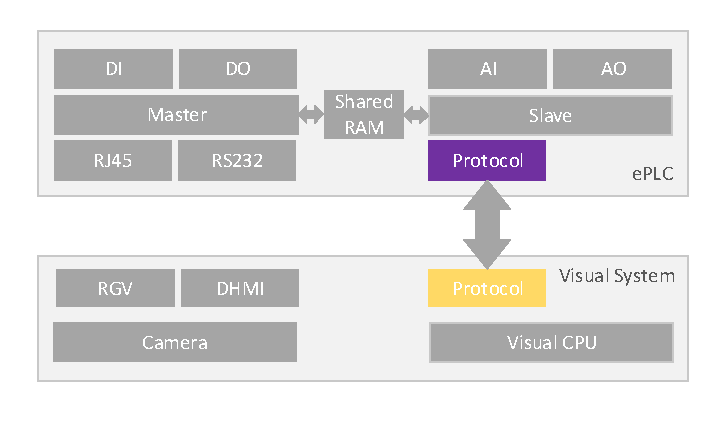
\includegraphics[width=3.5in]{fig/Hardware.pdf}
	\caption{A typical $ES$ which adopts two processor architecture. The shared memory is used to transfer data between master and slave processors. The communication between $ES$ and $VS$ adopt the CAN Bus.}
	\label{fig:Hardware}
\end{figure}
\subsection{Software Structure}
The typical software structure is seen as in Fig. \ref{fig:Software}. To our best knowledge, the $VS$ commonly contains several visual algorithms and every algorithm could extract some required parameters form pictures or videos. Meanwhile, the $ES$ is comprised of modules which conclude logic part and algorithms. The algorithms here are main motion control algorithms. Regarding the normal development method of visual servo control, the $VS$ and $ES$ is developed individually and using the communication protocol combines this two parts. However, this method should be always redesigned the programs in both systems because of the various visual algorithms and motion control algorithms. In addition, the logic and motion control are mixed together to develop in $ES$ and there are also lots of communication protocols (EtherCat, Modbus, Can, etc.). Considering the high complexity of today’s applications, it will be a cumbersome task.

Hence, we propose a multi-level flexible architecture which is based on $VCA$ protocol to address the problem of lack of generic method to integrate the $VS$ and $ES$. As shown in Fig. \ref{fig:Software}, the architecture contains three layers: flexible layer ($FL$), control layer ($CL$) and algorithm layer ($AL$).

\textbf{Flexible layer}: these layer is responsible for joint the $VS$ and $ES$ and consists of $PLC$ interface and visual interface. The parameters are framed with $VCA$ protocol frame (henceforth, abbreviated form of $PF$) interacted between $VS$ and $ES$. Furthermore, a special protocol template ($PT$) is saved in both systems to illustrate the protocol.

\textbf{Control layer}: this is independent of algorithm layer to cope with the logic tasks. This make it possible to run the logic task and algorithm task in different processors.

\textbf{Algorithm layer}: it is mainly comprised of types of algorithms which could be built in individual processors for algorithms with high performance requirement. 


\begin{figure}
	\centering
	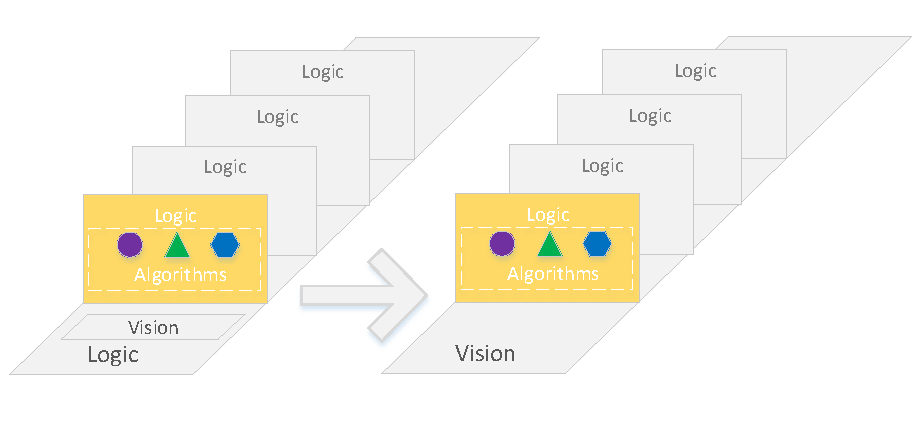
\includegraphics[width=3.5in]{fig/Software.pdf}
	\caption{Multi-level flexible architecture contains three layers: flexible layer, control layer and algorithm layer.}
	\label{fig:Software}
\end{figure}
%%%Fig.4. The three-layer architecture of embed PLC.



\subsection{Thread Structure}
We adopt the analogous thread structure in \cite{wu2018customized}. Three special threads introduced below:
\begin{enumerate}
	\item Visual Thread. This thread is responsible for interaction with $VS$. It will receive the protocol frame from the $VS$ and save it to relevant address. 
	\item Control Thread. Control thread mainly execute logic program, deframe the protocol frame and interaction data with algorithm thread.
	\item Algorithm Thread. Algorithm thread runs in slave processors. It is used to implement data interaction between processors and execution of algorithms.
\end{enumerate}

\begin{figure}
	\centering
	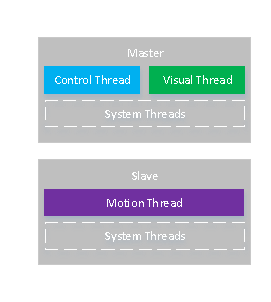
\includegraphics[width=3in]{fig/Threads.pdf}
	\caption{ Thread structureThe with three special threads: visual thread, Control thread, algorithm thread.}
	\label{fig:Threads}
\end{figure}
\subsection{Memory Allocation}
\begin{figure}
	\centering
	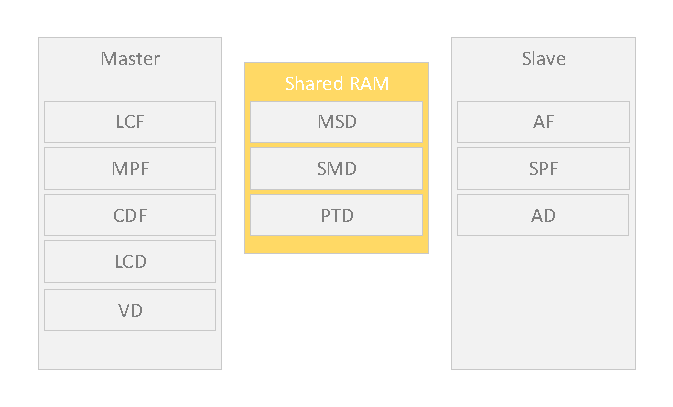
\includegraphics[width=3in]{fig/RAM.pdf}
	\caption{Memory allocation of master processor, shared ram and slave processor.}
	\label{fig:RAM}
\end{figure}
The dedicated storage area of $PLC$ in memory is made up of bit data area ($M$ area) and byte data area ($D$ area). Meanwhile, we regard $M$ area and $D$ area as set $M$ of bit and set $D$ of byte. Henceforth, we have three definitions below.

\textbf{Definition 1} If $\exists$ set $S$, we define its subscripted lowercase letter $s_i$ as an element of $S$ and the subscripted $i$ is used to distinguish the elements.

\textbf{Definition 2} If $\exists S \subseteq M$ and $(\forall s_{i} \in S) \in \{0, 1\} $. Meanwhile, each element $s_i$ has four operators: $\mathcal{S}_0(s_i)$ assigns $0$ to $s_i$, $\mathcal{S}_1(s_i)$ assigns $1$ to $s_i$, $\mathcal{J}_0(s_i)$ represents that the value of $s_i$ is $0$, $\mathcal{J}_1(s_i)$ means that the value of $s_i$ is $1$. Then we define the set $S$ has $\mathcal{B}$ attribute.

\textbf{Definition 3} If $\exists S \subseteq D$ and $\forall s_{i} \in S$ has 4 bytes. We define the set $S$ has $\mathcal{D}$ attribute.

Fig. \ref{fig:RAM} shows the memory allocation of master processor, shared RAM and slave processor. The shared $RAM$ is a special structure to fast data interaction between master and slave processors. In more general cases, the $MtoS$ is located in master processor, the $StoM$ is located in slave processor and the $PT$ is in both master and slave processors. 

\textbf{\emph{MCF}} (Module Control Flag Area): the flag are used to start the modules. It has $\mathcal{B}$ attribute.

\textbf{\emph{MPF}} (Master Processor Data Interaction Flag Area): it contains begin data transfer flag from master to slave ($MSB$), transfer state of master from master to slave ($MSF$), acknowledge flag of master from master to slave ($MSA$) and transfer state of master from slave to master ($MSS$). All of them have $\mathcal{B}$ attribute.


\textbf{\emph{MDF}} (Module data saved flag area): this flags denote whether the module data are saved. It has $\mathcal{B}$ attribute.

\textbf{\emph{LCD}} (Logic Control Data Area): these data will be used to store the control frame. It has $\mathcal{D}$ attribute. Every element $lcd_i$ is associated with a specified module.

\textbf{\emph{VD}} ($VCA$ protocol frame data area): all the frames received from the $VS$ are stored in this area.

\textbf{\emph{MSD}} (Master Processor Data Interaction Data Area): an area stores the data delivered from slave processors and it has $\mathcal{D}$ attribute.

\textbf{\emph{SMD}} (Slave Processor Data Interaction Data Area): an area stores the data delivered from master processor and it has $\mathcal{D}$ attribute.

\textbf{\emph{ADF}} (Algorithm data saved flag Area): the flags denote whether the algorithm data are saved. It has $\mathcal{B}$ attribute.

\textbf{\emph{PTD}} (Protocol Template Data Area): the protocol template is stored in this area and could be read by both processors.


\textbf{\emph{AF}} (Algorithm Flag Area): it includes algorithm flag of execution ($AFE$) and algorithm flag of state ($AFS$).
Both of them have $\mathcal{B}$ attribute.

\textbf{\emph{SPF}} (Slave Processor Data Interaction Flag Area): this area includes the begin data transfer flag from slave to master ($SMB$), transfer state of slave from slave to master ($SMF$), acknowledge flag of slave from slave to master ($SMA$) and transfer state of slave from master to slave ($SMS$). All of them have $\mathcal{B}$ attribute.

\textbf{\emph{AD}} (Algorithm Data Area): these data help specified algorithm executing. It has $\mathcal{D}$ attribute.
 
 We define the $\mathcal{P}$ to interact data between master processor and slave processor. It contains transferring data from master to slave ($\mathcal{P}_{mts}$) and transferring data from slave to master ($\mathcal{P}_{stm}$) which is defined below:
 \begin{equation}
 \left\{
 \begin{array}{l}
 \mathcal{P}_{mts} = \mathcal{U} (msb_i,msf_i,sma_i,sms_i,smd_i)\\
 \mathcal{P}_{stm} = \mathcal{U} (smb_i,smf_i,msa_i,mss_i,msd_i)
 \end{array}
 \right.
 \end{equation}
 Where $\mathcal{U}$ is the function to implement the process of data interaction between master and slave processors. $\mathcal{P}_{mts}$ and $\mathcal{P}_{mts}$ use the same function $\mathcal{U}$.
 
 The process of $\mathcal{P}_{mts}$ is seen below:
 	$\mathcal{S}_1(msb_i)\to\mathcal{S}_1(msf_i)\to send(smd_i)\to\mathcal{S}_0(msb_i)\to\mathcal{S}_1(sms_i)\to check(smd_i)\to\mathcal{S}_1(sma_i)\to\mathcal{S}_0(sms_i)\to\mathcal{S}_0(sma_i)\to\mathcal{S}_0(msf_i)$.
 
 Where $send(msd_i)$ means sending data to $msd_i$ in slave processor. $check(msd_i)$ means to check data of $msd_i$.

 

%%%Fig.6. Distribution of dedicated public data area.
\section{Integration of $VS$ and $ES$}
\label{Integration}

\subsection{$VCA$ $PT$}
\begin{figure}
\centering
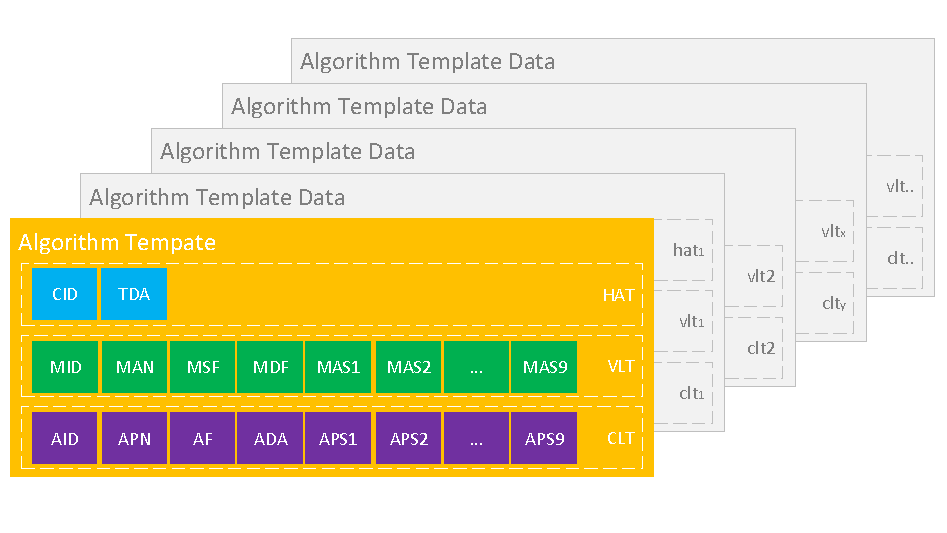
\includegraphics[width=3.5in]{fig/PT.pdf}
\caption{A $PT$ uniquely corresponds to a type of application. It contains four parts: head of protocol template, visual layer template , control layer template and algorithm layer template.}
\label{fig:PT}
\end{figure}
In cater to most applications, we propose a $VCA$ protocol based multi-level flexible architecture. As shown in Fig. \ref{fig:PT}, a protocol template ($PT$) is adopted to support various types of implementations and a $PT$ uniquely corresponds to a type of application. In the flexible architecture, users only need to redesign and reload the $PT$ and then they can reuse the visual servo system again. The $PT$ could be loaded into a stationary address of visual system and $ePLC$ system. After restarting both systems, it will be put into a fixed area of $RAM$. The parsing modules form both systems will read it when parsing the $PF$. The $VCA$ protocol could be used to bidirectionally transfer $PF$ using the same $PT$ and algorithms of framing and deframing.  
 
 The $PT$ is defined below:
  \begin{equation}
 \left\{
 \begin{array}{l}
 PT = \{HPT, VPT, APT, PPT\}\\
 HPT = \{CID, TDA\}\\
 VPT = \{MID, MAN, MDN, MDA, MSF, MDF, \\
 \qquad\qquad\quad \bigcup_{x=1}^i MAF_x, \bigcup_{x=1}^j CPS_x\}\\
 APT = \{AID, APN, ADA, AF, ADF, \bigcup_{y=1}^i APS_y\}\\
 PPT = \{PID, VID, VAR\}
 \end{array}
 \right.
 \end{equation}
 

 The $PT$ contains four parts: head of protocol template ($HPT$), VCA protocol template ($VPT$), algorithm protocol template ($APT$) and parameter protocol template ($PPT$). Every part explains as follows: 
 \begin{enumerate}
 	\item $HPT$: this part includes communication unique ID ($CID$), template data storage address ($TDA$). Every $PT$ only has one $HPT$.
 	\item $VPT$: it consists of module unique ID ($MID$), module contained algorithm number ($MAN$), , module contained data number ($MDN$), module data start address ($MDA$), module start flag ($MSF$), module data saved flag ($MDF$), module contained algorithm IDs ($MAS_x$) . $VLT$ is not $\emptyset$. Every $VPT$ includes $MAN$ algorithm IDs. 
 	\item $APT$: it is comprised of algorithm unique ID ($AID$), algorithm contained parameter number ($APN$), algorithm data start address $ADA$, algorithm data saved flag ($ADF$), algorithm contained parameter IDs ($APS_y$). $CLT$ is not $\emptyset$. Every $APT$ includes $APN$ parameter IDs.
 	\item $PPT$: it contains parameter unique ID ($PID$), its relevant visual algorithm ID ($VID$) and the conversion ratio of visual algorithm parameters and motion algorithm parameters ($VAR$).  
 \end{enumerate}
 \subsection{$VCA$ $PF$}
 The $VCA$ protocol frame ($PF$) contains parameter frames and algorithm frames in its data field and the algorithm protocol frame contains several parameter frames as shown in \ref{fig:Protocol}. 

 \begin{enumerate}
	\item $PF$: it consists items of $MID$, visual frame length ($VFL$), data from parameter frames ($PFDATA$) and data form algorithm frames($AFDATA$).The $PFDATA$ and $AFDATA$ contains several parameter frames and control frames, respectively. The $MID$s both in $PT$ and $PF$ need one-to-one correspondence.
	\item Algorithm frame: it is comprised of $AID$, control frame length ($CFL$) and $PFDATA$. The $AID$s both in algorithm frame and $PF$ need one-to-one correspondence.
	\item Parameter frame: it contains $PID$, $PDATA$. $PID$ is also the address of $PDATA$. The $PID$s both in parameter frame and $PF$ need one-to-one correspondence.
\end{enumerate}


\begin{figure}
	\centering
	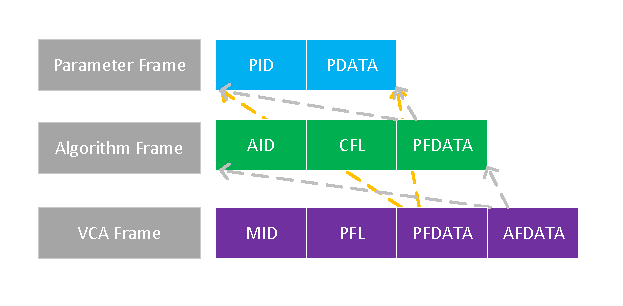
\includegraphics[width=3in]{fig/Protocol.pdf}
	\caption{ $VCA$ protocol frame contains parameter frames and algorithm frames in its data field and the algorithm protocol frame contains several parameter frames.}
	\label{fig:Protocol}
\end{figure}
\subsection{Framing of $PF$}
The framing contains three steps: $VCA$ framing, $CL$ framing, $AL$ framing. Transfer data ($TD$) save the data to be transferred and it is indexed by the $PID$. In the $VS$, it represents the parameters obtained form the visual algorithms. In the $ES$, the data come from the $RAM$.   


\textbf{\emph{VCA} Framing}: the process is realized as the Algorthm \ref{alg1}. It searches the $PT$ with $mid$ to find the relevant $vlt_x$. Through it, we can obtain the $man$ and $mdn$. According to $man$ and $mdn$, call the Algorithm \ref{alg3} and Algorithm \ref{alg2} to gain the $pfdata$ and $afdata$. Then calculate the length ($vfl$) to finish the $VCA$ framing.

\textbf{\emph{CL} Framing}: Algorthm \ref{alg2} illustrates the process. It seeks the $PT$ to gain the $alt_y$ which contains the $apn$. According to $apn$, call the Algorithm \ref{alg3} to obtain the $pfdata$ and then calculate the length ($cfl$) to finish the $AL$ framing.  

\textbf{\emph{P} Framing}: Algorthm \ref{alg3} shows the process. The $VS$ obtains the $alt_z$ frome $FT$ and then combines the $pid$ and $pdata$.


\begin{algorithm}
	\label{alg1}
	\caption{$VCAFraming$}%算法名字
	%\LinesNumbered %要求显示行号
	\KwIn{$mid$, $TD$}%输入参数
	\KwOut{$PF$}%输出
	SearchPT ($mid$, $vpt_x$)\;
	$PF.mid\leftarrow mid$\; 
	\For{$i=0$;$i<vpt_x.mdn$;$i++$}{
		ALFraming ($vpt_x$.$cps$[i], $TD$,$pfdata$)\;
	}
	\For{$i=0$;$i<vpt_x.man$;$i++$}{
		CLFraming ($vpt_x$.$mas$[i], $TD$,$afdata$)\;
	}
    $PF.pfdata\leftarrow$ $pfdata$\; 
    $PF.afdata\leftarrow$ $afdata$\; 
	$PF.vfl\leftarrow$ ($vpt_x.mdn+vpt_x.man$) $\times$ 4 + 8\;
\end{algorithm}

\begin{algorithm}
	\label{alg2}
	\caption{$CLFraming$}%算法名字
	%\LinesNumbered %要求显示行号
	\KwIn{$aid$, $TD$, $afdata$}%输入参数
	\KwOut{$afdata$}%输出
	SearchPT ($aid$, $apt_y$)\;
	Create $clf$\;
	$af.aid\leftarrow$ $aid$\;
	\For{$i=0$;$i<apt_y.apn$;$i++$}{
		ALFraming($apt_y$.$aps$[i], $TD$, $pfdata$)\;
	}
	$af.cfl \leftarrow$ $apt_y.apn \times 4$ + 8\;
	$af.pfdata \leftarrow$ $pfdata$\;	
	$afdata\leftarrow$ $afdata$ + $clf$\;	 
\end{algorithm}
\begin{algorithm}
	\label{alg3}
	\caption{$ALFraming$}%算法名字
	%\LinesNumbered %要求显示行号
	\KwIn{$pid$, $TD$,$pfdata$}%输入参数
	\KwOut{$pfdata$}%输出
	SearchPT ($pid$, $ppt_z$)\;
	Create $pf$\;
	$pf.pid\leftarrow$ $pid$\; %How to address the problem of id is same with address.
	$pf.pdata \leftarrow$ $TD[pid]\times ppt_z.var$\;
	$pfdata\leftarrow$ $pfdata$ + $alf$\;	 
\end{algorithm}

\subsection{Deframing of $PF$}
 The process of deframing of $PF$ has three parts: $VCA$ deframing, $CL$ deframing and $AL$ deframing. Received Data ($RD$) are used to save the deframing parameters. the $RD1$, $RD2$ and $RD3$ are different temporarily storing data area. In the $VS$,  $RD3$ are the data fed back to visual algorithms. In the $ES$, the $RD1$, $RD2$ and $RD3$ donate $LCD$, $MSD$ and $AD$, respectively.

\textbf{\emph{VCA} deframing}: as illustrated in Algorithm \ref{alg4}, obtain the $mid$ and $pfl$ form the start four and following four bytes data of $PDF$, respectively. Search the $PT$ to gain the relevant $vpt_x$. Send the $pfl-8$ bytes start form the eighth byte of $PDF+8$ to the address $mda$ of $vlt_x$.

\textbf{\emph{CL} deframing}: according to $mid$, search $PT$ to find the relevant $vpt_x$. Loop deal with the $mda$ times of the parameter frame. In each loop, the data are sent to $RD3$ with the relevant $pid$. Loop deal with the $man$ times of the algorithm frame. In each loop, use the $aid$ to find $apt_y$ and then send the $afdata$ to correlative address of $RD2$. Algorithm \ref{alg5} is described the process.

\textbf{\emph{AL} deframing}: use $aid$ to get its $apt_y$. Loop cope with the algorithm frame $apn$ times. Send the parameters to $RD3$ with the correlative $pid$. The process is shown in Algorithm \ref{alg6}.

\begin{figure}
	\centering
	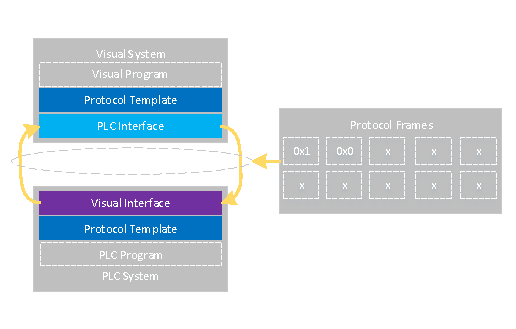
\includegraphics[width=3in]{fig/FlexibleLayer.pdf}
	\caption{ $PF$ interaction between PLC interface and visual interface.}
	\label{fig:FlexibleLayer}
\end{figure}
\begin{algorithm}
	\label{alg4}
	\caption{$VLDeframing$}%算法名字
	%\LinesNumbered %要求显示行号
	\KwIn{$PDF$}%输入参数
    $mid \leftarrow$ four bytes start form $PDF$\;
    searchPT ($mid$, $vpt_x$)\;
    $pfl \leftarrow$ four bytes start form $PDF+4$\; 
    $RD1[vpt_x.mda]\leftarrow$ $pfl-8$ bytes start form $PDF+8$\;     	
	$PDF\leftarrow$ $PDF+pfl$\;
\end{algorithm}

\begin{algorithm}
	\label{alg5}
	\caption{$CLDeframing$}%算法名字
	%\LinesNumbered %要求显示行号
	\KwIn{$mid$}%输入参数
	searchPT($mid$, $vpt_x$)\;
	$mda\leftarrow$ $vpt_x.mda$\;	
	\For{$i=0$;$i<vpt_x.mdn$;$i++$}{
		$RD3[RD1[mda]]\leftarrow$ 4 bytes start form $mda+4$\;
		$mda\leftarrow mda+8$\;
	}
	\For{$i=0$;$i<vpt_x.man$;$i++$}{
		searchPT($vpt_x.mas[i]$, $apt_y$)\;
		$RD2[apt_y.apa]\leftarrow$ $apt_y.vfl - 8$ bytes start form $mda+8$\; 
        $mda\leftarrow$ $mda+apt_y.vfl$\;
	}
\end{algorithm}

\begin{algorithm}
	\label{alg6}
	\caption{$ALDeframing$}%算法名字
	%\LinesNumbered %要求显示行号
	\KwIn{$aid$}%输入参数
	searchPT($aid$, $apt_y$)\;
	$ada\leftarrow$ $apt_y.ada$\;
	\For{$i=0$;$i<apt_y.apn$;$i++$}{
		$RD3[RD2[ada]]\leftarrow$ 4 bytes start form $ada+4$\;
		$ada\leftarrow ada+8$\;
	}
\end{algorithm}


\section{System Operation Mechanism}
\label{Execution}
\subsection{Implementation of Flexible Program and Execution}
The $FL$ contains two parts: $PLC$ interface and visual interface, shown in Fig. \ref{fig:FlexibleLayer}. They interact with each other using the agreed communication protocol which is defined as $CID$ in $HPT$ of $PT$. The execution from PLC interface to visual interface is comprised of five steps.  

The $PLC$ interface is responsible for get parameters of motion control form $VS$ and interact with $ES$. It includes three steps blew.

\textbf{Step 1}: after image processing, the $VS$ extracts the useful data and stores into data required to be transfered ($TD$) in which the parameters could be indexed by the $PID$.

\textbf{Step 2}: frame $TD$ into $PF$ with the Algorithm \ref{alg1}, \ref{alg2} and \ref{alg3}. Here, the $TD$ is an array in $VS$.

\textbf{Step 3}: transfer the $PF$s to $ePLC$ with the relevant communication protocol in $CID$.

\textbf{Step 4}: visual interface receives $PF$s from $VS$ according the $CID$ in $HPT$.

\textbf{Step 5}: visual interface saves them in the $ES$. There are two pointers: $PDF$ and $PSP$, shown in Fig. \ref{fig:VisualInterface}. $PDF$ points to the address of deframing $PF$ and $PSP$ points to the address of saving $PF$. The $PDF$ will point to the next address of $PF$ if a $PF$ is deframed. After saved the $PF$, the $PSP$ will point to the next new address according the $vfl$ of $PF$. 

The execution from visual interface to PLC interface consists of the following steps.
\textbf{Step 1}: visual interface frames $TD$ into $PF$ with the Algorithm \ref{alg1}, \ref{alg2} and \ref{alg3}. Here, the $TD$ is in $RAM$ of $ePLC$.

\textbf{Step 2}: visual interface transfers the $PF$s to $VS$ with the relevant communication protocol in $CID$.

\textbf{Step 3}: PLC interface deframes the $PF$s with the Algorithm \ref{alg4}, \ref{alg5} and \ref{alg6}.
\begin{figure}
	\centering
	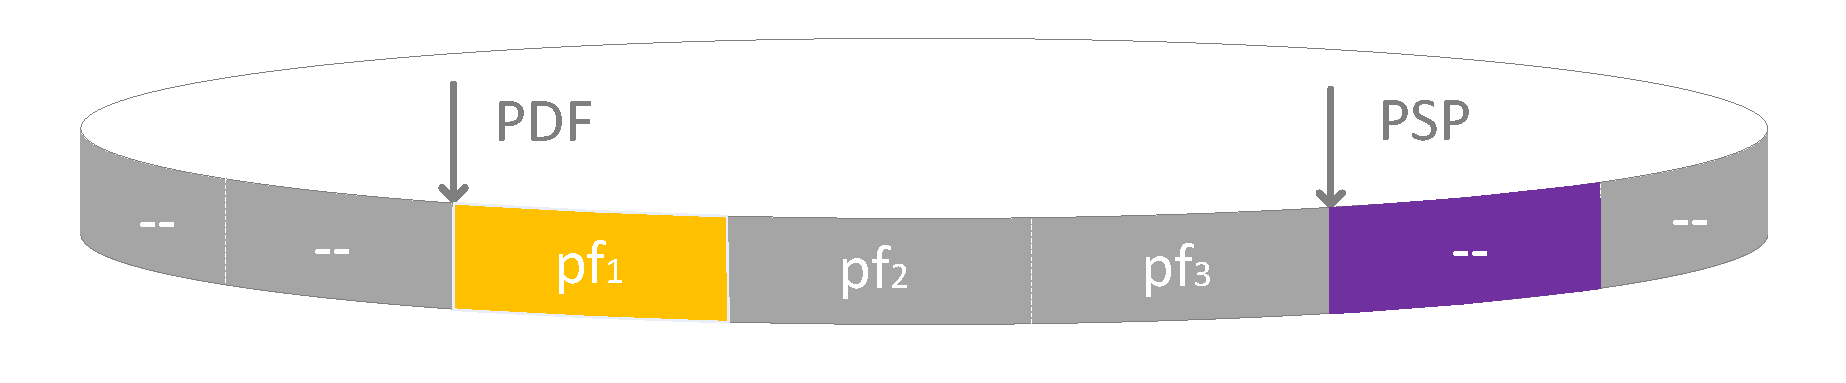
\includegraphics[width=3in]{fig/VisualInterface.pdf}
	\caption{ $PDF$ and $PSP$. $PDF$ points to the address of deframing $PF$ and $PSP$ points to the address of saving $PF$. The $PDF$ will point to the next address of $PF$ if a $PF$ is deframed. After saved the $PF$, the $PSP$ will point to the next new address according the $vfl$ of $PF$.}
	\label{fig:VisualInterface}
\end{figure}

%\begin{figure}
%	\centering
%	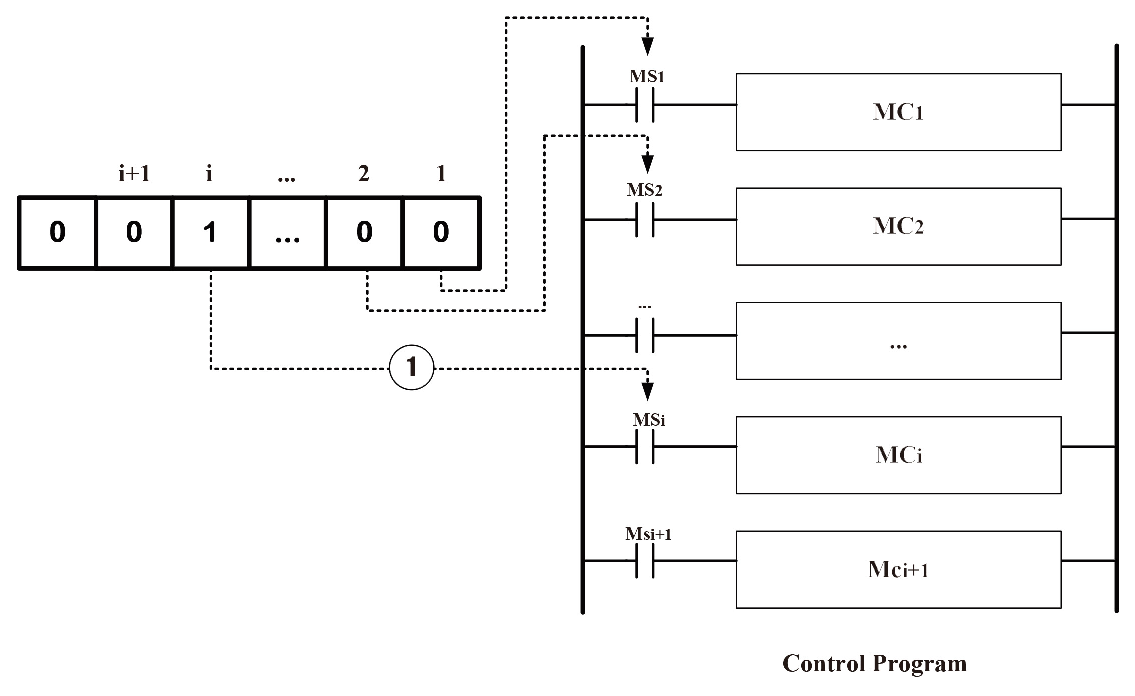
\includegraphics[width=3.5in]{fig/bitdatainM.eps}
%	\caption{Using bit data in the M area to control program module$\textquoteright$s execution}
%	\label{fig:bitdatainM}
%\end{figure}
%%%Fig.11. Using bit data in M area to control program module¡¯s execution.


\subsection{Implementation of Control Program and Execution}
Control program $CP$ is responsible for organizing the modules, executing the logic program, deframing the $PF$ and interacting the data with algorithm program. $CP=\{VLDP,CLDP, IP, LP, PIP\}$, where $CLP$ is the control layer deframe program. $IP$ is the initial program which is used to initialize the data and state. $LP$ is the logic program. $PIP$ is the processor interaction program implemented to transfer and receive data between processors. The implementation of control program is described below.

\textbf{Step 1}: if the pointer $PDF!=PSP$, execute the $VLDP$ which means to call Algorithm \ref{alg4}.

\textbf{Step 2}: traverse the $LCF$ to check whether there is a module needed to execute. If $\exists$ $\forall$ $lcf_i \in LCF$ is 1, go to step 3.

\textbf{Step 3}: execute the $IP$ to initialize the data and state and then execute the $LP$ to find the called algorithm. If $\exists$ $\forall$ $af_i \in AF$ is 1, go to step 4. 

\textbf{Step 4}: if $\exists$ $\forall$ $adf_i \in ADF$ is 1, execute the $CLDP$ to call Algorithm \ref{alg5}, go to step 5. 

\textbf{Step 5}: the $\mathcal{P}_{mts}$ is used in $PIP$ to inform the slave processor to receive parameters and start algorithms and clear the relevant $af_i$.   

\textbf{Step 6}: read and process the feedback data form the slave processor. 


%\begin{figure}
%\centering
%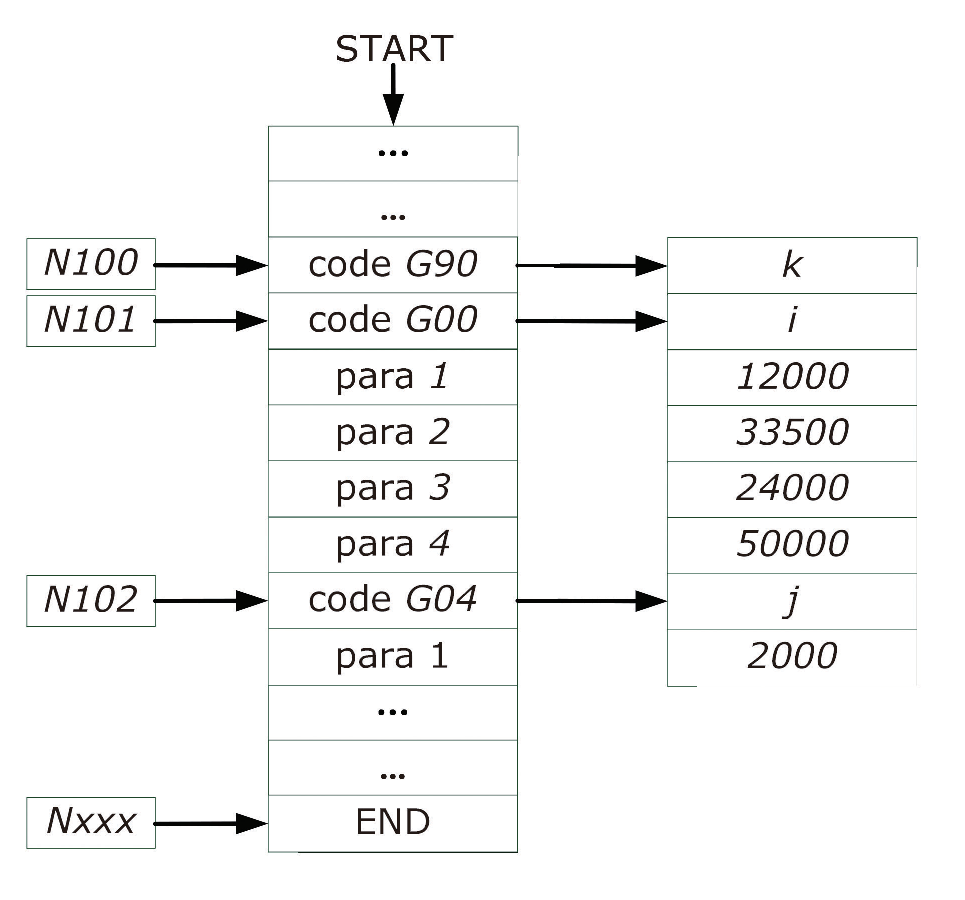
\includegraphics[width=3in]{fig/formatofCNCprogram.eps}
%\caption{The format of ACP program frame after compiling}
%\label{fig:formatofCNCprogram}
%\end{figure}
%%%Fig.8. The format of ACP program frame after compiling.




%%%Fig.9. The schematic of delivering ACP instruction parameters from ACPDD to ACPPSD

%\begin{figure}
%	\centering
%	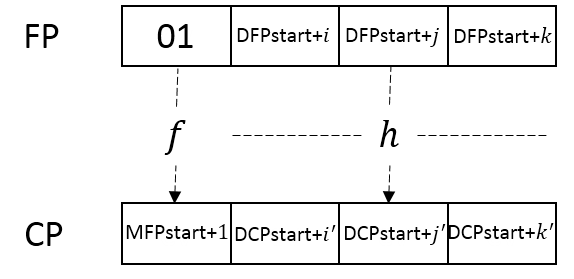
\includegraphics[width=2.5in]{fig/compilation.png}
%	\caption{ The compilation from flexible program to control program}
%	\label{fig:compilation}
%\end{figure}

%\begin{figure}
%	\centering
%	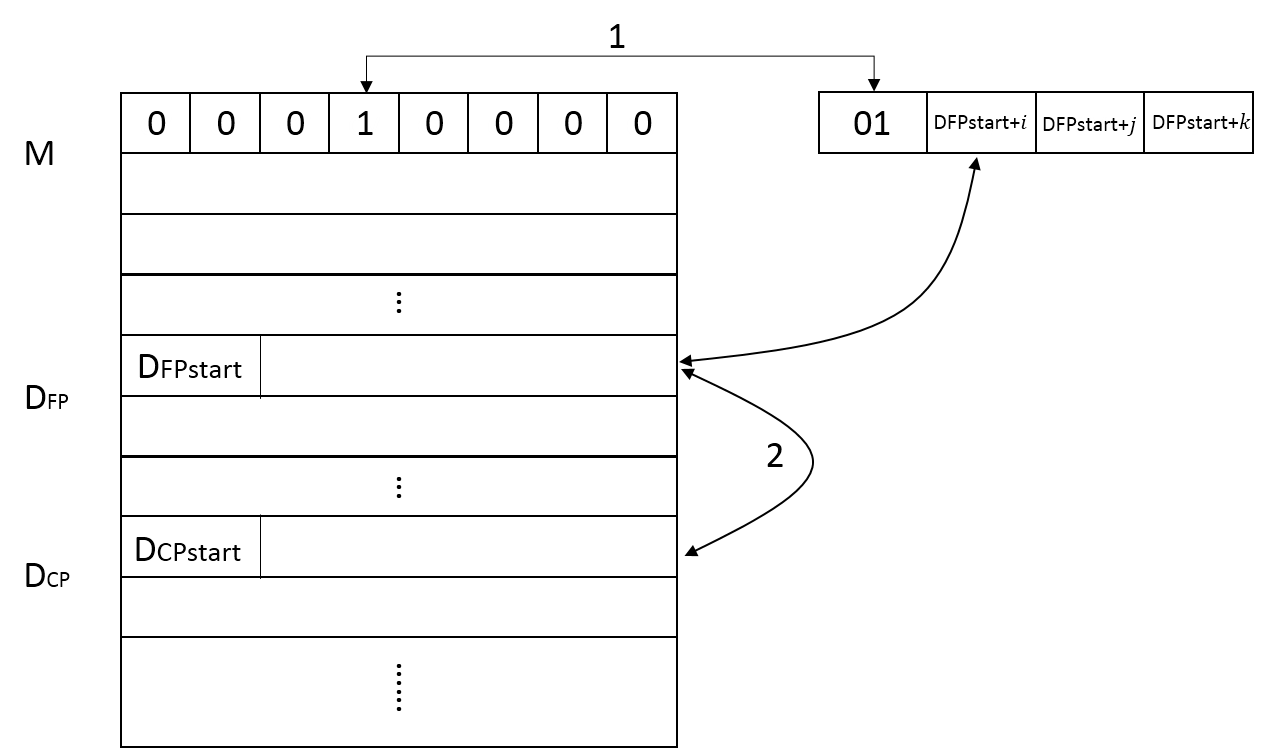
\includegraphics[width=2.5in]{fig/DataTransfer.png}
%	\caption{ The compilation from flexible program to control program}
%	\label{fig:DataTransfer}
%\end{figure}

%\begin{figure}
%	\centering
%	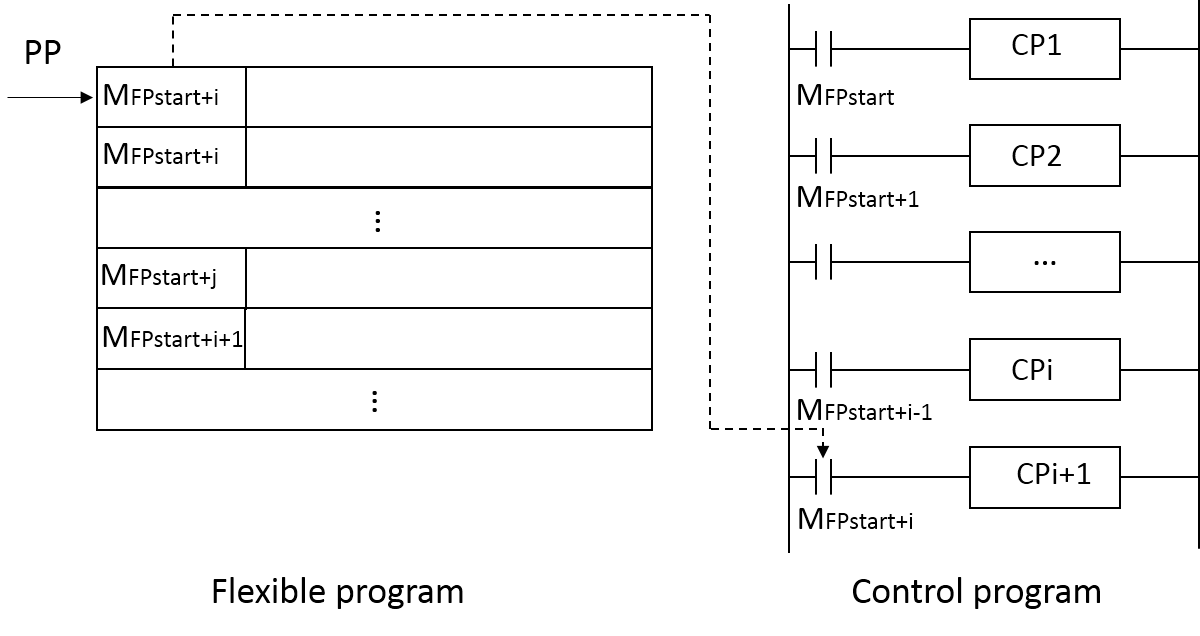
\includegraphics[width=3in]{fig/execution.png}
%	\caption{ The execution OF flexible program}
%	\label{fig:execution}
%\end{figure}

\subsection{Implementation and Execution of Algorithm Program }
The Algorithm Program ($AP$) is in $EL$. $AP=\{\mathcal{P}_{stm}, AS, ALDP\}$, where $\mathcal{P}_{stm}$ feeds back data to master processor, $AS$ contains all algorithms and $ALDP$ deframe the $AL$ frame. The execution of algorithm program is introduced below.

\textbf{Step 1}: traverse the $LCF$ to check whether there is a algorithm needed to execute. If $\exists$ $\forall$ $af_i \in AF$ is 1, go to step 2.

\textbf{Step 2}: if $\exists$ $\forall$ $adf_i \in ADF$ is 1, $ALDP$ is executed to call Algorithm \ref{alg5}, go to step 3. 

\textbf{Step 3}: execute the motion algorithm.

\textbf{Step 4}: the $\mathcal{P}_{stm}$ is used to feed back data to the master processor. 

\subsection{Execution of Threads}
 Commonly, threads in master processor and in slave processors execute separately according to their priority and the interaction between control thread and algorithm threads occurs when using $\mathcal{P}_{mts}$ and $\mathcal{P}_{mts}$. 
 
 Visual thread consists of the following units.
 
 \textbf{$V_1$}: receive $PF$ from $VS$ with the agreed communication protocol.
 
 \textbf{$V_2$}: check $PF$ and store it into $VD$. 
 
 \textbf{$V_3$}: call Algorithm \ref{alg4} to deframe the $PF$ and saved the $cdata$ into $LCD$.
 
 Basic execution units of control thread are shown as follows:

\textbf{$C_{1}$}: start a module and initial it.

\textbf{$C_{2}$}: run logic program. 

\textbf{$C_{3}$}: call Algorithm \ref{alg5} to deframe control frame.

\textbf{$C_{4}$}: transfer data to slave processor by $\mathcal{P}_{mts}$.

\textbf{$C_{5}$}: deal with the feedback data.

\textbf{$C_{6}$}: end the module.

Motion thread contains the following basic execution units:

\textbf{$M_{1}$}: Start a algorithm.

\textbf{$M_{2}$}: Call Algorithm \ref{alg6} to deframe the algorithm frame.

\textbf{$M_{3}$}: Execute the algorithm.

\textbf{$M_{4}$}: Feedback the data to master processor by $\mathcal{P}_{stm}$.

\textbf{$M_{5}$}: End the algorithm.

The threads execute as shown in Fig. \ref{fig:threadExecution}. Visual thread ($VT$) continuously executes the unit $V1$ if there exits $PF$ from $VS$, executes unit $V2$ to store the $PF$ into $VD$ at the address of $PSP$ and execute $V3$ to deframe $PF$ at the address of $PDF$ and store its $cdata$ into $LCD$ and $\mathcal{S}_1 {cdf_i}$.
The control thread ($CT$) traverses $LCF$, finds $\exists \mathcal{J}_1 {lcf_i}$ and then executes the unit $C1$, executes unit $C_2$. If find a required execution algorithm and $\exists$ its $\mathcal{J}_1 {mdf_j}$ then $CT$ starts unit $C3$ to deframe the control frame and then runs unit $C4$ and inform algorithm thread ($AT$) to execute $M_1$ unit. Next, $AT$ executes unit $M2$ transferring data from $SMD$ to $AD$. After that, the unit $M3$ is executed. During the running of algorithm, the unit $M4$ is continuously executed to feed data back to $CT$, meanwhile $CT$ will execute unit $C5$ to response it until the execution of $M5$ and no other executed algorithms neither. During the running of the module, if the $VT$ receives new $PF$ and $CT$ finds $\exists \mathcal{J}_1 {cdf_i}$, $CT$ will execute unit $C_3$ and $C_4$ again. Next, the $VT$ will run unit $M_2$ to update the parameters. If the $MT$ finished all algorithms, then $CT$ will run unit $C_6$ to finished the module and continue to traverse the $LCF$ to find another required execution module.   

\begin{figure}
	\centering
	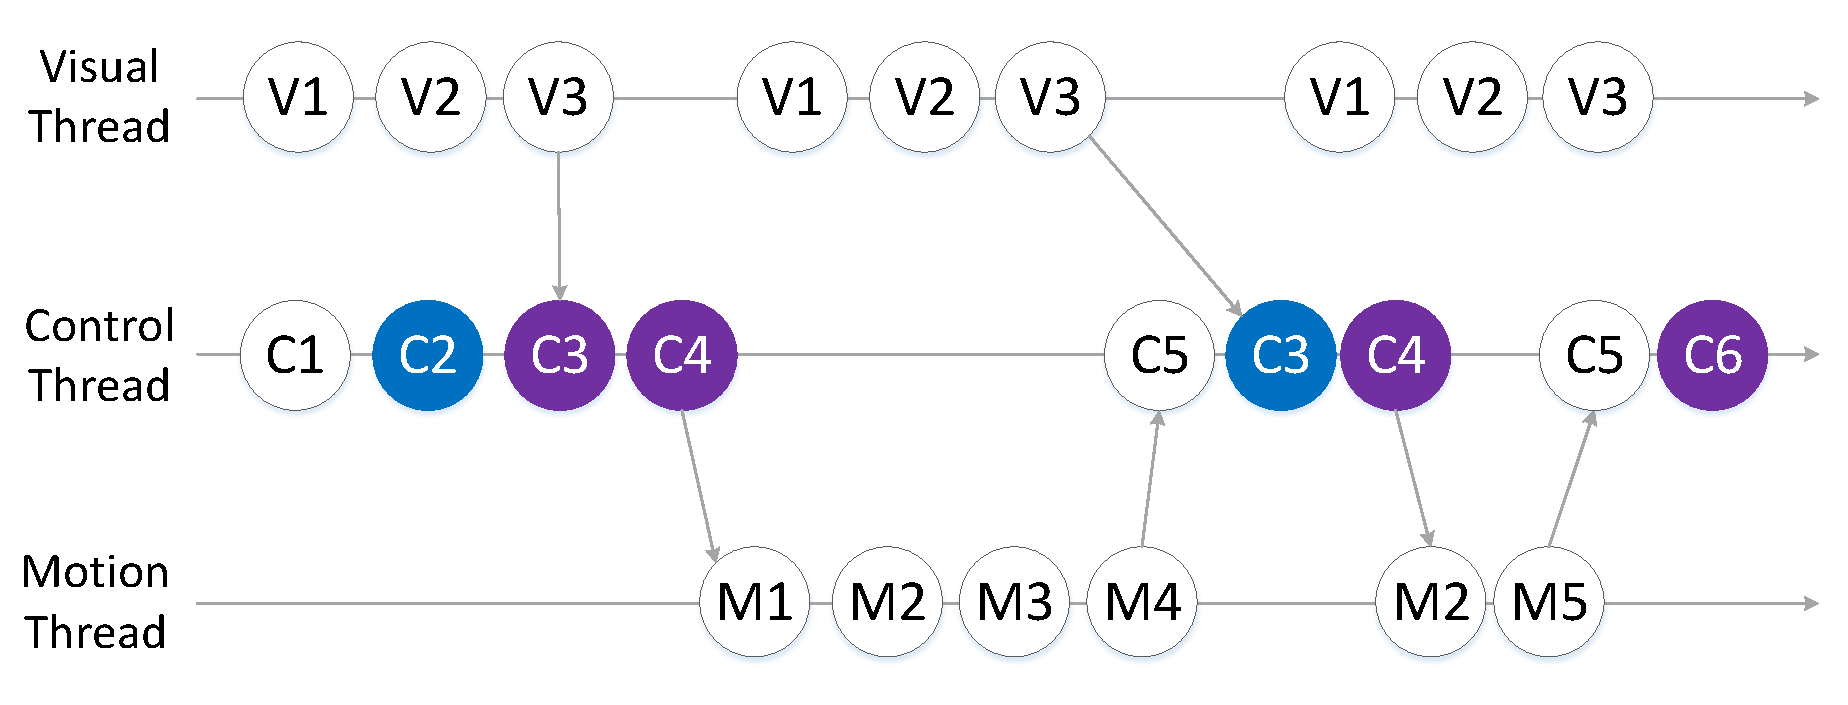
\includegraphics[width=3in]{fig/ThreadExecution.pdf}
	\caption{ Process of thread execution.}
	\label{fig:threadExecution}
\end{figure}

\section{Case Analysis}
\label{Case}
In this section, we introduce two scenarios of the proposed $VCA$ protocol based integration method in ePLC. With the $VCA$ protocol, users only need to code additional algorithms and change the $PT$ when the scenario of visual servo system is changed. 

\subsection{Case 1: Winding Machine with Visual System}
  
As shown in Fig. \ref{fig:Winding}, (a) is the visual system, whose CUP is ARM9 based S3C2440 and which uses the CANIF interface to communicate with OV9650 CMOS Camera; (b) is the $ePLC$, CASS-PLCA149B; (c) is the winding machine with visual system which contains two axes: the U-axis and Q-axis; (d) is shown the Winding effect, the angle of the wire, Q-axis and U-axis. In winding process, the tension of the copper wire will change irregularly, especially for the thick ones. However, we use the same speed ratio of U-axis and Q-axis which always leads to irregularity of each layer of the coil. Hence, we can use the visual system to decrease or increase the speed of Q-axis to control the angle of wire. 

Fig. \ref{fig:WindingSystem} is the structure of the winding machine system. The ePLC has two chips: a master chip and a slave chip. It uses the RS232 to receive $PF$s and could control six servo systems at most. The winding machine has two axes: the U-axis and Q-axis. The $VS$ use the CMOS camera to gain winding images and transfer the digital information to ARM CUP. The ARM CUP will extract parameters from the digital information, frame $PF$s and transfer $PF$s to $ePLC$ continuously. 


\subsubsection{Design of $PT$}
In \cite{wu2018customized}, we propose the customized winding machine language which only contains 13 instructions. Here, we can use the second and third instructions to control U-axis and Q-axis, respectively.The process of winding is mainly to control the speed ratio of U-axis and Q-axis, hence we use the $VS$ to influence the speed of Q-axis only. The $PT$ of winding machine is illustrated in Table \ref{table:PTofWinding} in which the $pid_1$ is the speed of Q-axis and the 1000 of $var_1$ is used to multiply by the $\theta$.
\begin{table}
	\scriptsize \caption{$PT$ of winding machine}
	\label{table:PTofWinding}
	\begin{center}
		\renewcommand{\arraystretch}{1.4}
		\setlength\tabcolsep{3pt}
		\begin{tabular}{|p{1cm}|p{1cm}|p{1cm}|p{1cm}|p{1cm}|p{1cm}|p{1cm}|}
			\hline
			$cid_1$  & $tda_1$   &xxx &xxx& xxx  &xxx &xxx \\
			\hline
			0x01&0x00&& &&&\\
			\hline
			$mid_1$   & $man_1$ &$mdn_1$ &$mda_1$&$msf_1$& $mdf_1$  & $mas_1$\\
			\hline
			0x01      & 1     &   0    &0X200   &0X400   & 0X600  &0x01 \\
			\hline
			$aid_1$  & $apn_1$& $af_1$ &$ada_1$ &$aps1_1$  &xxx&xxx\\
			\hline
			0x01     & 0X1    & 0X14A  &0x1F4000 &0X0   & &\\
			\hline
			$pid_1$  &$vid_1$ &$var_1$ &xxx      &xxx   &xxx &xxx\\
            \hline
			0X0      & 0X1    & 1000   &         &   & &\\
	    	\hline
		\end{tabular}
	\end{center}
\end{table}
\subsubsection{Process of $PF$}
Table \ref{table:PFofWinding} is shown the interacted $PF$ between the $VS$ and $ES$. At first, the $VS$ detects that the $\theta$ is 2 degrees. Then, it sends the $PF$ to inform the $ES$ to increase the Q-axis speed of 2000 pulses per millisecond (p/ms). When the $\theta$ decreases to 1 degree, the increment of the Q-axis speed is changed to 1000 p/ms. Since the $\theta$ has recovered to 0, the $ES$ is informed to recover the initial speed if the Q-axis.  
\begin{table}
	\scriptsize \caption{$PF$ of winding machine}
	\label{table:PFofWinding}
	\begin{center}
		\renewcommand{\arraystretch}{1.4}
		\setlength\tabcolsep{3pt}
		\begin{tabular}{|p{1.2cm}|p{1.2cm}|p{1.2cm}|p{1.2cm}|p{1.2cm}|p{1cm}|}
			\hline
			$mid_1$   & $pfl_1$ &$aid_1$ & $cfl_1$  & $pid_1$  &$pdata_1$   \\
			\hline
			0x01    & 0x14  &0x01  &0xE     &0x01   &0x400   \\
			\hline
			0x01    & 0x14  &0x01  &0xE     &0x01   &0x200   \\
			\hline
			0x01    & 0x14  &0x01  &0xE     &0x01   &0x000   \\
			\hline
		\end{tabular}
	\end{center}
\end{table}
\begin{figure}
	\centering
	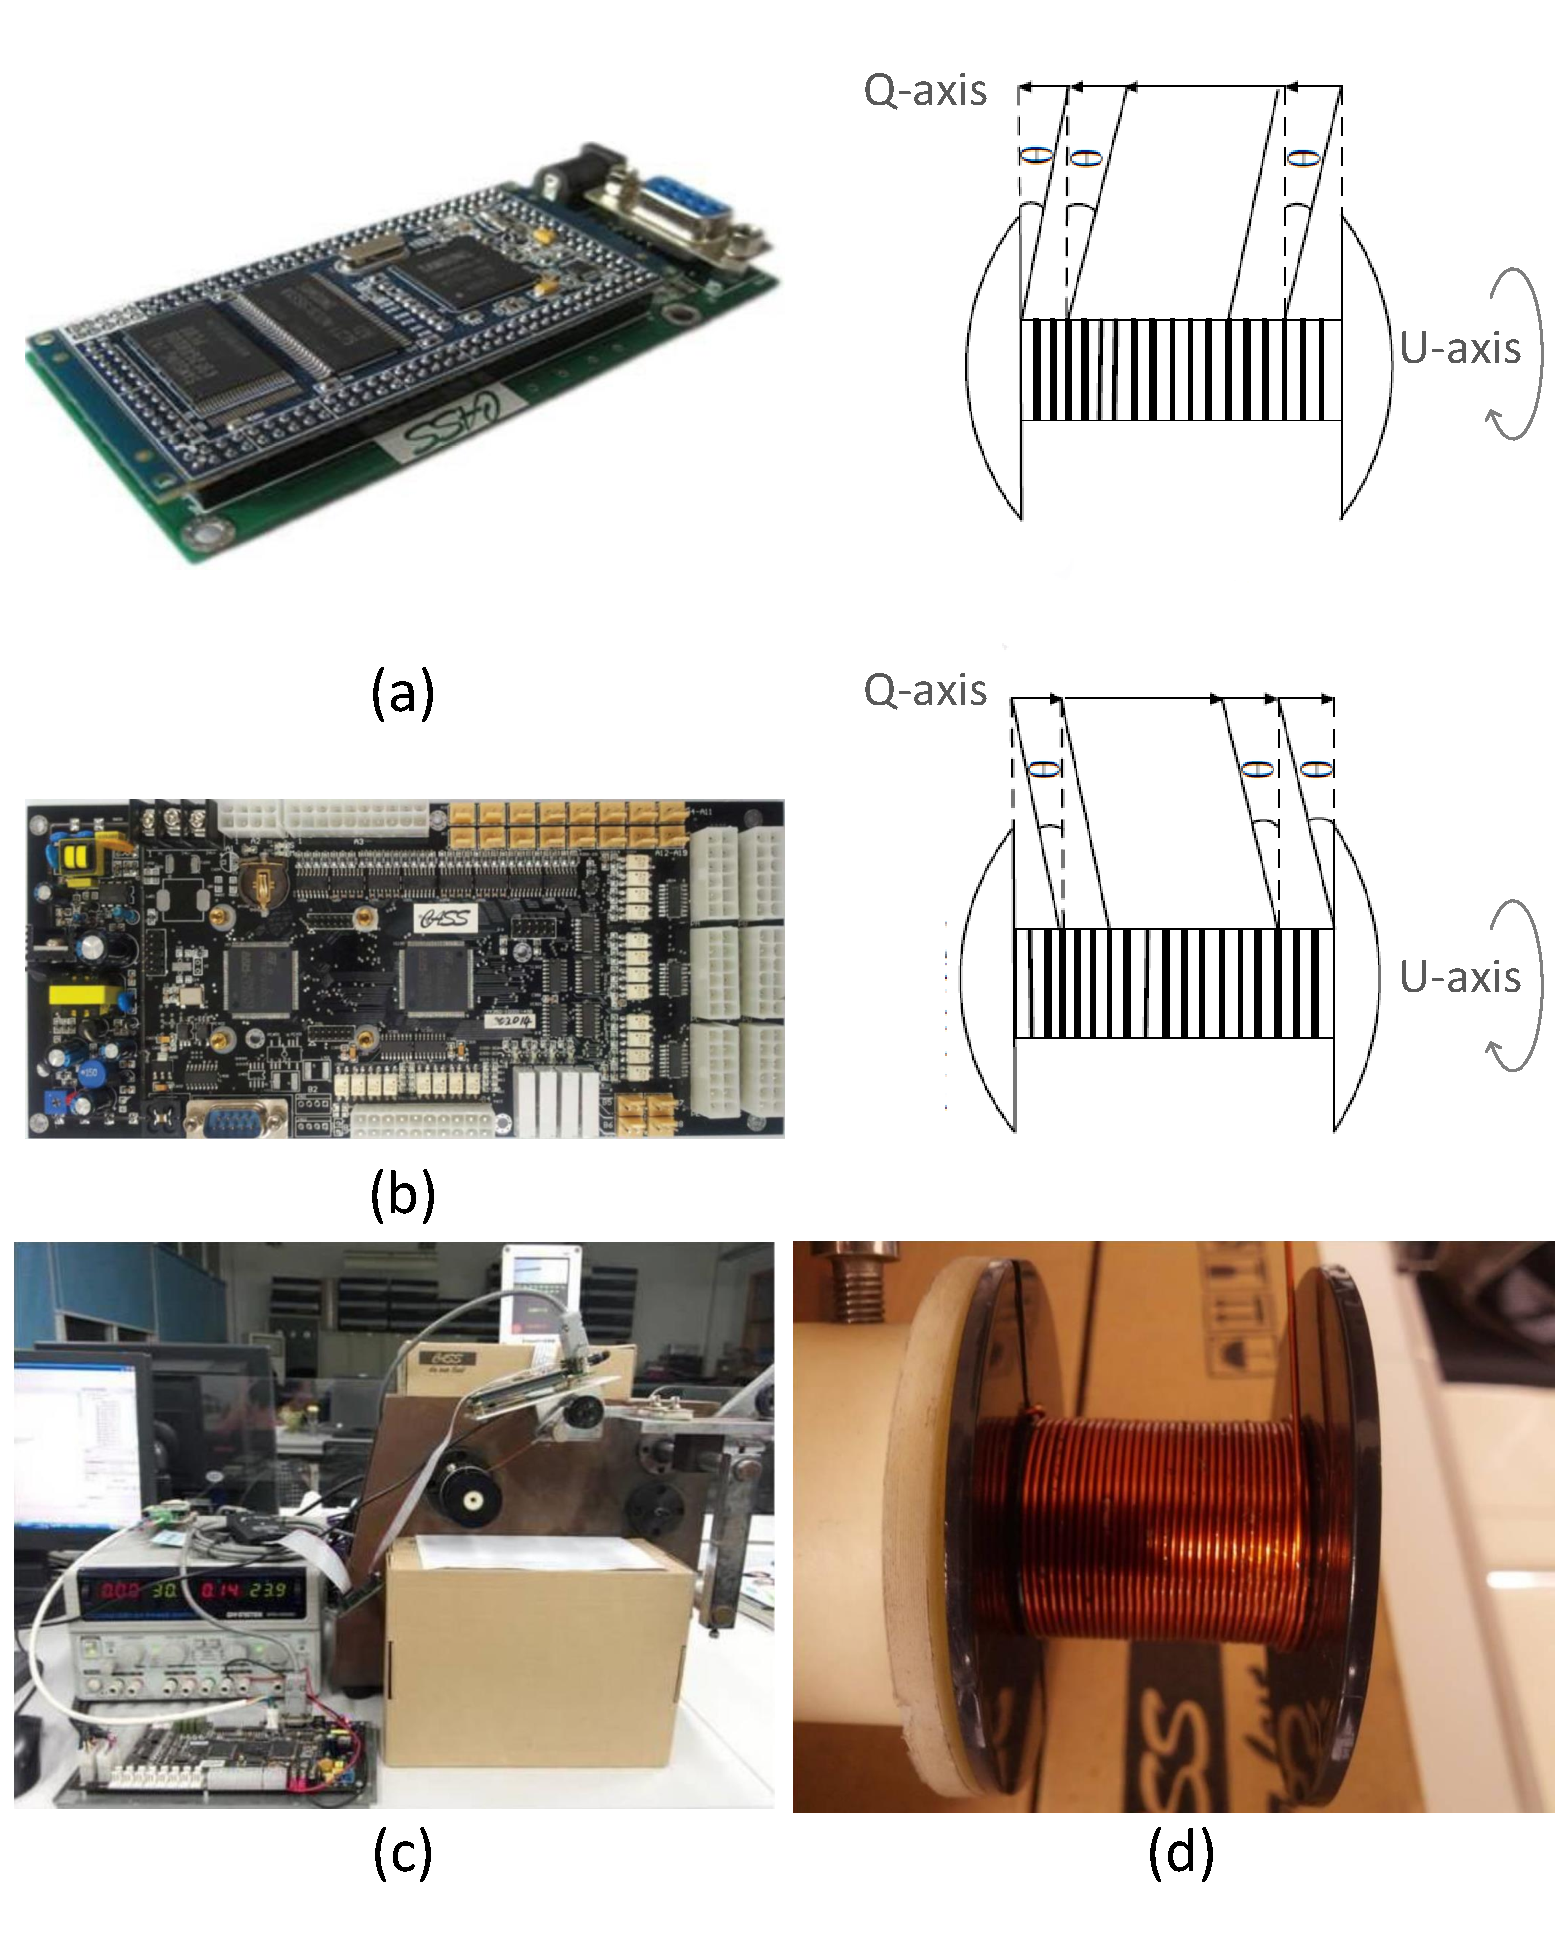
\includegraphics[width=3in]{fig/Winding.pdf}
	\caption{ (a) is the visual system, whose CUP is ARM9 based S3C2440 and which uses the CANIF interface to communicate with OV9650 CMOS Camera; (b) is the $ePLC$, CASS-PLCA149B; (c) is the winding machine with visual system which contains two axes: the U-axis and Q-axis; (d) is shown the Winding effect, the angle of the wire, Q-axis and U-axis.}
	\label{fig:Winding}
\end{figure}
\begin{figure}
	\centering
	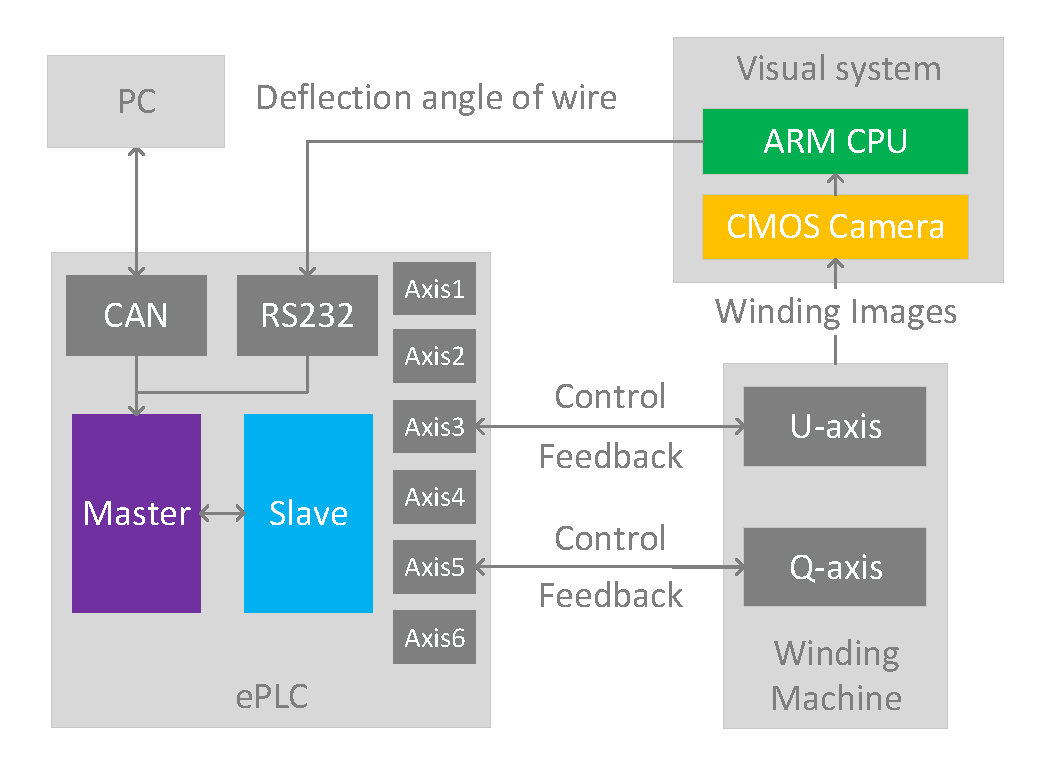
\includegraphics[width=3in]{fig/WindingSystem.pdf}
	\caption{ Structure of the winding machine system. The ePLC has two chips: a master chip and a slave chip. It uses the RS232 to receive $PF$s and could control six servo systems at most. The winding machine has two axes: the U-axis and Q-axis. The $VS$ use the CMOS camera to gain winding images and transfer the digital information to ARM CUP. The ARM CUP will extract parameters, frame $PF$s and transfer them to $ePLC$ continuously.}
	\label{fig:WindingSystem}
\end{figure}
\subsection{Case 2: Binocular Catching Robot}
\begin{figure}
	\centering
	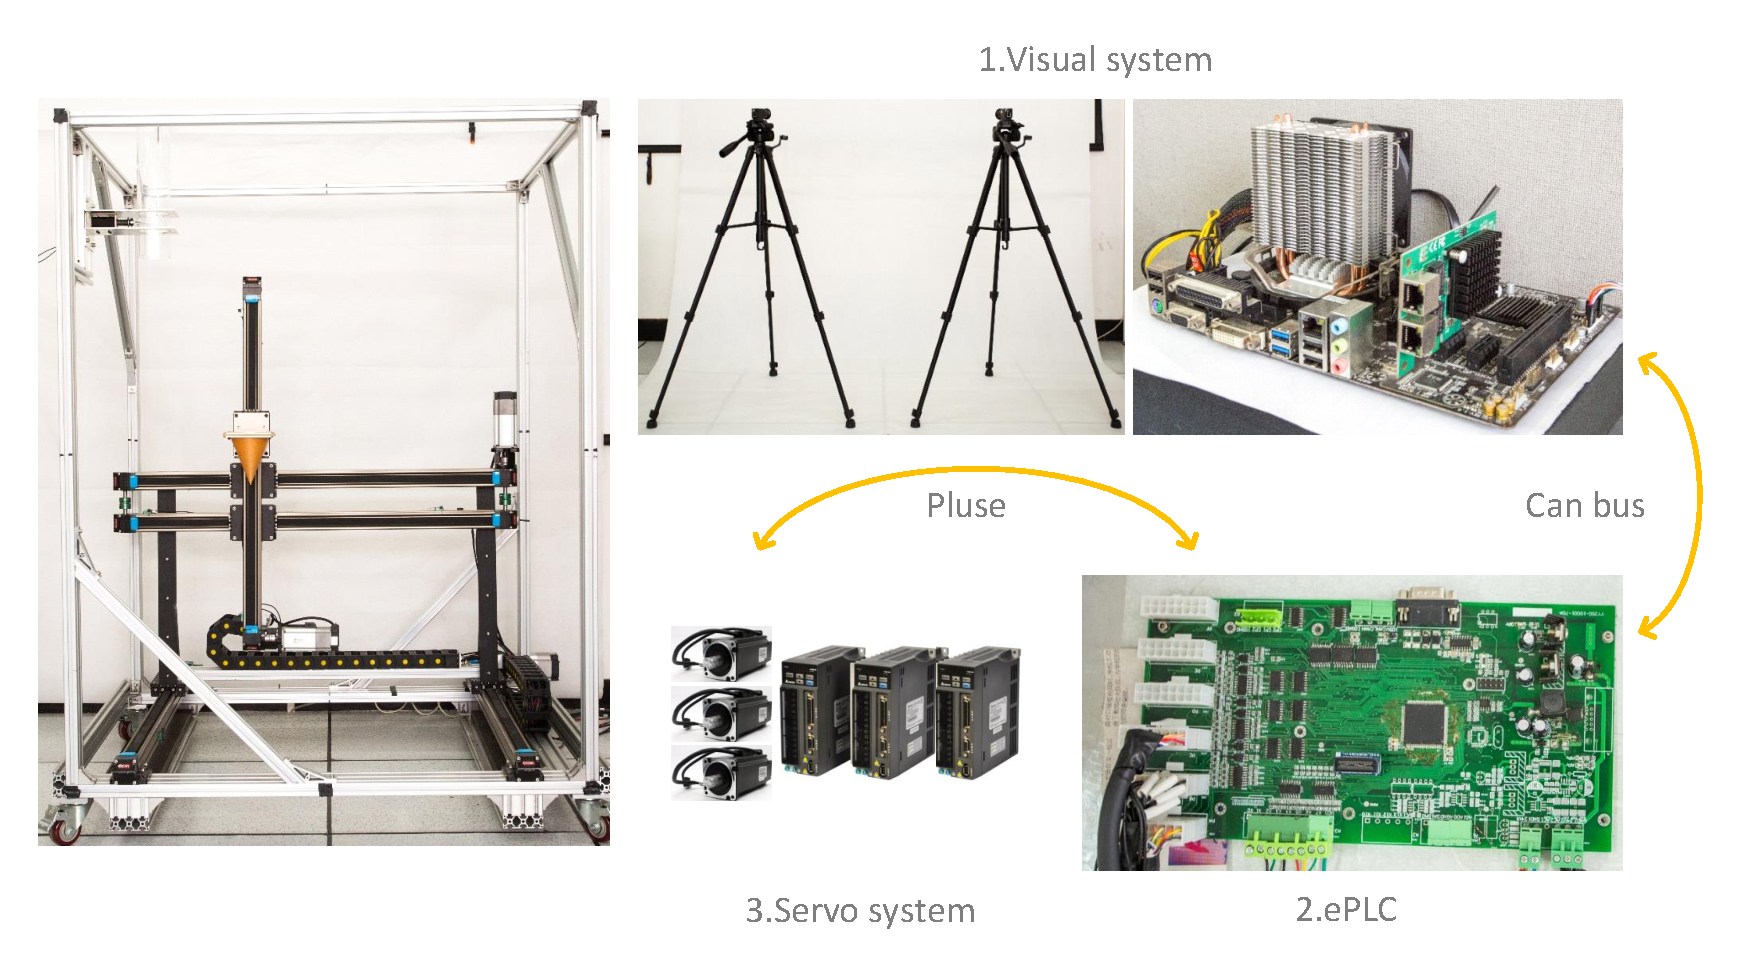
\includegraphics[width=3in]{fig/robot.pdf}
	\caption{ Binocular Catching Robot consists of visual system, $ePLC$ and servo system.}
	\label{fig:robot}
\end{figure}
As shown in Fig. \ref{fig:robot}, the binocular catching robot adopts two cameras to judge the position of the ball in the space. Through sending the continuously parameters to $ePLC$, the robot runs to the position to catch the ball. Finally, the robot will catch the ball. The cameras is xxx, the visual system is xxx. $ePLC$ uses the TI F28M35 chip with two cores: ARM Cortex M3 and TI C28x, which contains a shared RAM. The servo system is adopted ASDA-B2. 
\subsubsection{Design of $PT$}
The $ePLC$ is designed to control six axes parallel. We adopt the same algorithm of Q-axis and U-axis in case one while we name three axes of the Cartesian Robot as X-axis, Y-axis and Z-axis. In this case, we have the similar module with case one however it contains three motion algorithms. $pid_1$, $pid_2$ are the position and speed of X-axis; $pid_3$, $pid_4$ are the position and speed of Y-axis; $pid_5$, $pid_6$ are the position and speed of Z-axis. The $VS$ use meter and meter per second (m/s) to measure the distance and speed, respectively while in the $ES$, driving every 1 cm need to output 10000 pluses. Hence, the $VAR$ of position and speed are both 10000.    
\begin{table}
	\scriptsize \caption{$PT$ of binocular catching robot}
	\label{table:PTofRobot}
	\begin{center}
		\renewcommand{\arraystretch}{1.4}
		\setlength\tabcolsep{3pt}
		\begin{tabular}{|c|c|c|c|c|c|c|c|c|}
			\hline
			$cid_1$  & $tda_1$   &xxx &xxx& xxx  &xxx &xxx&xxx&xxx \\
			\hline
			0x01&0x00&& &&&&&\\
			\hline
			$mid_1$  &$man_1$&$mdn_1$&$mda_1$&$msf_1$&$mdf_1$&$mas_1$&$mas_1$&$mas_1$\\
			\hline
			0x01     &1     &   0    &0X200  &0X400  & 0X600 &0x01   &0x02   &0x03 \\
			\hline
			$aid_1$  & $apn_1$& $af_1$ &$ada_1$ &$aps1_1$  &$aps2_1$&xxx&xxx&xxx\\
			\hline
			0x01     & 0X2    & 0X14A  &0x1F4000 &0X0   &0x4 &&&\\
			\hline
			$aid_2$  & $apn_2$& $af_2$ &$ada_2$ &$aps1_2$  &$aps2_2$&xxx&xxx&xxx\\
			\hline
			0x02     & 0X2    & 0X14A  &0x1F4000&0X8       &0xA &&&\\
			\hline
			$aid_3$  & $apn_3$& $af_3$ &$ada_3$ &$aps1_3$  &$aps2_3$&xxx&xxx&xxx\\
			\hline
			0x03     & 0X2    & 0X14A  &0x1F4000&0XE       &0X10 &&&\\
			\hline
			$pid_1$  &$vid_1$ &$var_1$ &$pid_2$ &$vid_2$&$var_2$ &$pid_3$&$vid_3$&$var_3$\\
			\hline
			0X0      & 0X1    & 10000  &0X4     &0X1    & 10000  &0X8      & 0X1    & 10000\\
			\hline
			$pid_4$  &$vid_4$ &$var_4$ &$pid_5$ &$vid_5$&$var_5$ &$pid_6$  &$vid_6$ &$var_6$\\
			\hline
			0XA      & 0X1    & 10000  &0XE     &0X1    & 10000  &0X10     & 0X1    & 10000\\
			\hline
		\end{tabular}
	\end{center}
\end{table}


\begin{table*}
	\scriptsize \caption{$PF$ of binocular catching robot}
	\label{table:PFofrotot}
	\begin{center}
		\renewcommand{\arraystretch}{1.4}
		\setlength\tabcolsep{3pt}
		\begin{tabular}{|c|c|c|c|c|c|c|c|c|c|c|c|c|c|c|c|c|c|c|c|}
			\hline
			$mid_1$   & $pfl_1$ 
			&$aid_1$  & $cfl_1$  & $pid_1$  &$pdata_1$ & $pid_2$  &$pdata_2$
			&$aid_2$  & $cfl_2$  & $pid_3$  &$pdata_3$ & $pid_4$  &$pdata_4$
			&$aid_3$  & $cfl_3$  & $pid_5$  &$pdata_5$ & $pid_6$  &$pdata_6$  \\
			\hline
			0x01    & 0x14  
			&0x01  &0xE     &0x01   &0x400   &0x01   &0x400 
			&0x01  &0xE     &0x01   &0x400   &0x01   &0x400
			&0x01  &0xE     &0x01   &0x400   &0x01   &0x400\\
			\hline
			0x01    & 0x14  
			&0x01  &0xE     &0x01   &0x400   &0x01   &0x400  
			&0x01  &0xE     &0x01   &0x400   &0x01   &0x400
			&0x01  &0xE     &0x01   &0x400   &0x01   &0x400\\
			\hline
			0x01    & 0x14  
			&0x01  &0xE     &0x01   &0x400   &0x01   &0x400  
			&0x01  &0xE     &0x01   &0x400   &0x01   &0x400
			&0x01  &0xE     &0x01   &0x400   &0x01   &0x400\\
			\hline
			0x01    & 0x14  
			&0x01  &0xE     &0x01   &0x400   &0x01   &0x400  
			&0x01  &0xE     &0x01   &0x400   &0x01   &0x400
			&0x01  &0xE     &0x01   &0x400   &0x01   &0x400\\
			\hline
			0x01    & 0x14  
			&0x01  &0xE     &0x01   &0x400   &0x01   &0x400  
			&0x01  &0xE     &0x01   &0x400   &0x01   &0x400
			&0x01  &0xE     &0x01   &0x400   &0x01   &0x400\\
			\hline
			0x01    & 0x14  
			&0x01  &0xE     &0x01   &0x400   &0x01   &0x400  
			&0x01  &0xE     &0x01   &0x400   &0x01   &0x400
			&0x01  &0xE     &0x01   &0x400   &0x01   &0x400\\
			\hline			
		\end{tabular}
	\end{center}
\end{table*}
\subsubsection{Process of $PF$}
The $PF$s of a time catching the ball is shown in Table \ref{table:PFofrotot} and the trajectory of the ball is shown in Fig. \ref{fig:Trajectory} which is only shown the position of X-axis and Y-axis. The $VS$ sends the $PF$ to $ES$ to adjust the destination and speed of every axis.

\begin{figure}
	\centering
	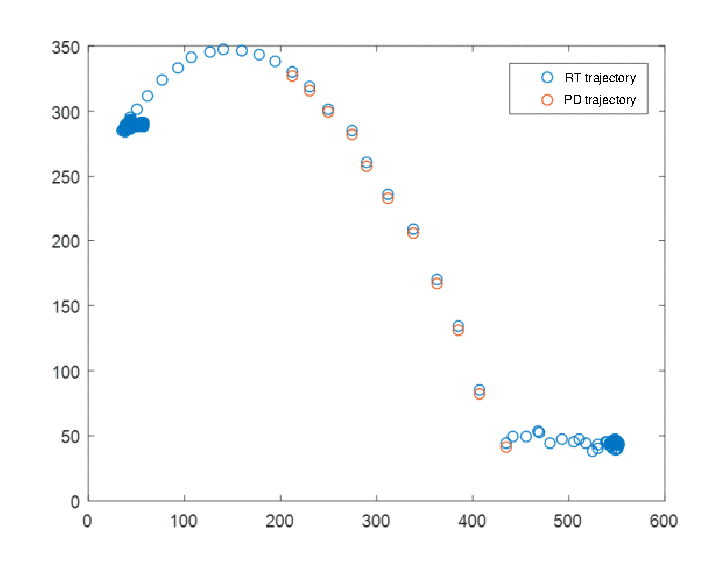
\includegraphics[width=3.5in]{fig/PFofRobot.pdf}
	\caption{ Trajectory of the ball which is only shown the position of X-axis and Y-axis.}
	\label{fig:Trajectory}
\end{figure}

\subsection{Result}
Through the analysis of two cases, the proposed $VCA$ based flexible structure provides a generic method to address the visual servo control problem in $ePLC$.  
\section{Conclusion}
\label{conclusion}
We propose a flexible multi-level architecture which is based on a $VCA$ protocol to address the problem of integration of PLC system, motion control system and visual system in ePLCs. The multi-level includes flexible layer, control layer and algorithm layer. The $VCA$ protocol is designed to data interaction between the layers. Correspondingly, a customized hardware, memory allocation, multithreading structure are described to support the proposed flexible software architecture.

In the further research, we will implement a uniform development method of the visual servo control in ePLC.

\ifCLASSOPTIONcaptionsoff
  \newpage
\fi



% trigger a \newpage just before the given reference
% number - used to balance the columns on the last page
% adjust value as needed - may need to be readjusted if
% the document is modified later
%\IEEEtriggeratref{8}
% The "triggered" command can be changed if desired:
%\IEEEtriggercmd{\enlargethispage{-5in}}

% references section

% can use a bibliography generated by BibTeX as a .bbl file
% BibTeX documentation can be easily obtained at:
% http://www.ctan.org/tex-archive/biblio/bibtex/contrib/doc/
% The IEEEtran BibTeX style support page is at:
% http://www.michaelshell.org/tex/ieeetran/bibtex/
%\bibliographystyle{IEEEtran}
% argument is your BibTeX string definitions and bibliography database(s)
%\bibliography{IEEEabrv,../bib/paper}
%
% <OR> manually copy in the resultant .bbl file
% set second argument of \begin to the number of references
% (used to reserve space for the reference number labels box)

\bibliographystyle{IEEEtran}
\bibliography{reference}

% biography section
%
% If you have an EPS/PDF photo (graphicx package needed) extra braces are
% needed around the contents of the optional argument to biography to prevent
% the LaTeX parser from getting confused when it sees the complicated
% \includegraphics command within an optional argument. (You could create
% your own custom macro containing the \includegraphics command to make things
% simpler here.)
%\begin{IEEEbiography}[{\includegraphics[width=1in,height=1.25in,clip,keepaspectratio]{mshell}}]{Michael Shell}
% or if you just want to reserve a space for a photo:

%\begin{IEEEbiography}[{\includegraphics[width=1in,height=1.25in,clip,keepaspectratio]{fig/Author_HuifengWu.eps}}]{Huifeng Wu} received the Ph.D. degree in computer science and technology from Zhejiang university, Hangzhou, China, in 2006. He is currently a professor in the institute of intelligent and software Technology, Hangzhou Dianzi University. His research interests include software development methods and tools, software architecture, embedded system, intelligent control \& automation.
%	
%\end{IEEEbiography}
%\begin{IEEEbiography}[{\includegraphics[width=1in,height=1.25in,clip,keepaspectratio]{fig/Author_YiYan.eps}}]{Yi Yan} received B.S. in automatic control engineering form Zhejiang Sci-Tech University in 1984, M.S. in computer engineering from Beijing University of Postal Telecommunications in 1990. Currently he is the director and full professor in institute of intelligent and software Technology, Hangzhou Dianzi University. His research interests include embedded system, advanced manufacturing system, intelligent control \& automation, and intelligent instruments.
%	
%	
%\end{IEEEbiography}
%\begin{IEEEbiography}[{\includegraphics[width=1in,height=1.25in,clip,keepaspectratio]{fig/Author_DanfengSun.eps}}]{Danfeng Sun} received M.S. in computer architecture from Hangzhou DianZi University in 2011. He is currently a research assistant in the Institute of Industrial Internet, Hangzhou DianZi University. His research interests include embeded system, motion control and IIoT.
%\end{IEEEbiography}
%\begin{IEEEbiography}[{\includegraphics[width=1in,height=1.25in,keepaspectratio,angle=-90]{fig/Author_ReneSimon.eps}}]{Rene Simon} obtained a doctor of engineering at the Otto-von-Guericke University Magdeburg in 2001. He is Professor of Control Systems at the Department of Automation and Computer Sciences, Harz University of Applied Sciences, Wernigerode, Germany. His major research fields include engineering of automation systems, especially industrial controllers. He is chairman of PLCopen and project leader IEC 61131-10 Ed. 1.0.
%\end{IEEEbiography}



% insert where needed to balance the two columns on the last page with
% biographies
%\newpage


% You can push biographies down or up by placing
% a \vfill before or after them. The appropriate
% use of \vfill depends on what kind of text is
% on the last page and whether or not the columns
% are being equalized.

%\vfill

% Can be used to pull up biographies so that the bottom of the last one
% is flush with the other column.
%\enlargethispage{-5in}



% that's all folks
\end{document}


